\documentclass[tikz,border=2pt]{standalone}
\usepackage{amsmath,amssymb}
\usetikzlibrary{arrows.meta,positioning}
\begin{document}
% The three parts of a GLM: linear predictor eta_i = x_i^T beta, inverse link mu_i = g^{-1}(eta_i),
% exponential-family response with mean mu_i and variance phi V(mu_i); log-link example eta_i = log 2 gives mu_i = 2.
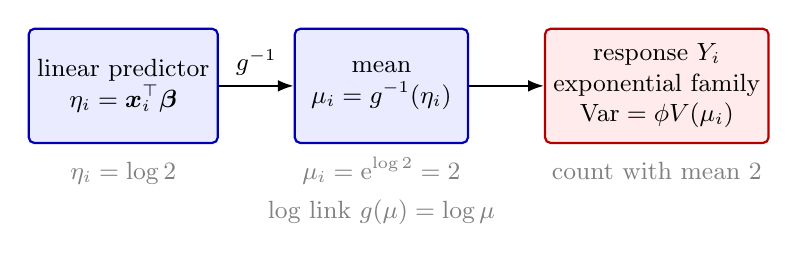
\begin{tikzpicture}[font=\small, >={Latex[length=2mm]},
    box/.style={draw, thick, rounded corners=2pt, align=center, minimum height=1.45cm, inner sep=3pt}]
  \node[box, draw=blue!70!black, fill=blue!8, minimum width=2.4cm] (eta) {linear predictor\\$\eta_i=\boldsymbol{x}_i^{\top}\boldsymbol{\beta}$};
  \node[box, draw=blue!70!black, fill=blue!8, minimum width=2.2cm, right=0.95cm of eta] (mu) {mean\\$\mu_i=g^{-1}(\eta_i)$};
  \node[box, draw=red!70!black, fill=red!8, minimum width=2.6cm, right=0.95cm of mu] (y) {response $Y_i$\\exponential family\\$\operatorname{Var}=\phi V(\mu_i)$};
  \draw[->, thick] (eta) -- node[above] {$g^{-1}$} (mu);
  \draw[->, thick] (mu) -- (y);
  % log-link example on one baseline
  \path (y.south) ++(0,-0.45) coordinate (b);
  \node[gray, anchor=base] at (b -| eta) {$\eta_i=\log 2$};
  \node[gray, anchor=base] at (b -| mu) {$\mu_i=\mathrm{e}^{\log 2}=2$};
  \node[gray, anchor=base] at (b -| y) {count with mean $2$};
  \node[gray, anchor=base] at ([yshift=-0.5cm]b -| mu) {log link $g(\mu)=\log\mu$};
\end{tikzpicture}
\end{document}
